\documentclass{article}

%%%% packages and definitions (optional)
\usepackage{graphicx} % allows inclusion of graphics
\usepackage{graphics}
\usepackage{booktabs} % nice rules (thick lines) for tables
\usepackage{microtype} % improves typography for PDF
\usepackage{xspace}
\usepackage[hidelinks]{hyperref}
\usepackage{xspace}

\newcommand{\SN}{S$_N$}
\renewcommand{\vec}[1]{\bm{#1}} %vector is bold italic
\newcommand{\vd}{\bm{\cdot}} % slightly bold vector dot
\newcommand{\grad}{\vec{\nabla}} % gradient
\newcommand{\ud}{\mathop{}\!\mathrm{d}} % upright derivative symbol
\newcommand{\Cyclus}{\textsc{Cyclus}\xspace}%
\graphicspath{ {images/} }
\usepackage[affil-it]{authblk}
\usepackage{tikz}
\usetikzlibrary{positioning, arrows, decorations, shapes }
\usepackage{cleveref}


\usepackage[acronym,toc]{glossaries}
%\newacronym{<++>}{<++>}{<++>}
\newacronym[longplural={metric tons of heavy metal}]{MTHM}{MTHM}{metric ton of heavy metal}
\newacronym{ABM}{ABM}{agent-based modeling}
\newacronym{ACDIS}{ACDIS}{Program in Arms Control \& Domestic and International Security}
\newacronym{ADS}{ADS}{Accelerator-Driven Systems}
\newacronym{AFCI}{AFCI}{Advanced Fuel Cycles Initiative}
\newacronym{AHTR}{AHTR}{Advanced High Temperature Reactor}
\newacronym{ANDRA}{ANDRA}{Agence Nationale pour la gestion des D\'echets RAdioactifs, the French National Agency for Radioactive Waste Management}
\newacronym{ANL}{ANL}{Argonne National Laboratory}
\newacronym{ANS}{ANS}{American Nuclear Society}
\newacronym{API}{API}{application programming interface}
\newacronym{ARE}{ARE}{Aircraft Reactor Experiment}
\newacronym{ARFC}{ARFC}{Advanced Reactors and Fuel Cycles}
\newacronym{ASME}{ASME}{American Society of Mechanical Engineers}
\newacronym{ASTRID}{ASTRID}{Advanced Sodium Technological Reactor for Industrial Demonstration}
\newacronym{ATWS}{ATWS}{Anticipated Transient Without Scram}
\newacronym{BDBE}{BDBE}{Beyond Design Basis Event}
\newacronym{BIDS}{BIDS}{Berkeley Institute for Data Science}
\newacronym{BWR}{BWR}{Boiling Water Reactor}
\newacronym{CAFCA}{CAFCA}{ Code for Advanced Fuel Cycles Assessment }
\newacronym{CDTN}{CDTN}{Centro de Desenvolvimento da Tecnologia Nuclear}
\newacronym{CEA}{CEA}{Commissariat \`a l'\'Energie Atomique et aux \'Energies Alternatives}
\newacronym{CI}{CI}{continuous integration}
\newacronym{CNEN}{CNEN}{Comiss\~{a}o Nacional de Energia Nuclear}
\newacronym{CNERG}{CNERG}{Computational Nuclear Engineering Research Group}
\newacronym{COSI}{COSI}{Commelini-Sicard}
\newacronym{COTS}{COTS}{commercial, off-the-shelf}
\newacronym{CSNF}{CSNF}{commercial spent nuclear fuel}
\newacronym{CTAH}{CTAHs}{Coiled Tube Air Heaters}
\newacronym{CUBIT}{CUBIT}{CUBIT Geometry and Mesh Generation Toolkit}
\newacronym{CURIE}{CURIE}{Centralized Used Fuel Resource for Information Exchange}
\newacronym{DAG}{DAG}{directed acyclic graph}
\newacronym{DANESS}{DANESS}{Dynamic Analysis of Nuclear Energy System Strategies}
\newacronym{DBE}{DBE}{Design Basis Event}
\newacronym{DESAE}{DESAE}{Dynamic Analysis of Nuclear Energy Systems Strategies}
\newacronym{DHS}{DHS}{Department of Homeland Security}
\newacronym{DOE}{DOE}{Department of Energy}
\newacronym{DRACS}{DRACS}{Direct Reactor Auxiliary Cooling System}
\newacronym{DRE}{DRE}{dynamic resource exchange}
\newacronym{DSNF}{DSNF}{DOE spent nuclear fuel}
\newacronym{DYMOND}{DYMOND}{Dynamic Model of Nuclear Development }
\newacronym{EBS}{EBS}{Engineered Barrier System}
\newacronym{EDF}{EDF}{Électricité de France}
\newacronym{EDZ}{EDZ}{Excavation Disturbed Zone}
\newacronym{EIA}{EIA}{U.S. Energy Information Administration}
\newacronym{EPA}{EPA}{Environmental Protection Agency}
\newacronym{EPR}{EPR}{European Pressurized Reactor}
\newacronym{EP}{EP}{Engineering Physics}
\newacronym{EU}{EU}{European Union}
\newacronym{FCO}{FCO}{Fuel Cycle Options}
\newacronym{FCT}{FCT}{Fuel Cycle Technology}
\newacronym{FEHM}{FEHM}{Finite Element Heat and Mass Transfer}
\newacronym{FEPs}{FEPs}{Features, Events, and Processes}
\newacronym{FHR}{FHR}{Fluoride-Salt-Cooled High-Temperature Reactor}
\newacronym{FLiBe}{FLiBe}{Fluoride-Lithium-Beryllium}
\newacronym{FP}{FP}{Fission Products}
\newacronym{GDSE}{GDSE}{Generic Disposal System Environment}
\newacronym{GDSM}{GDSM}{Generic Disposal System Model}
\newacronym{GENIUSv1}{GENIUSv1}{Global Evaluation of Nuclear Infrastructure Utilization Scenarios, Version 1}
\newacronym{GENIUSv2}{GENIUSv2}{Global Evaluation of Nuclear Infrastructure Utilization Scenarios, Version 2}
\newacronym{GENIUS}{GENIUS}{Global Evaluation of Nuclear Infrastructure Utilization Scenarios}
\newacronym{GPAM}{GPAM}{Generic Performance Assessment Model}
\newacronym{GRSAC}{GRSAC}{Graphite Reactor Severe Accident Code}
\newacronym{GUI}{GUI}{graphical user interface}
\newacronym{HLW}{HLW}{high level waste}
\newacronym{HPC}{HPC}{high-performance computing}
\newacronym{HTC}{HTC}{high-throughput computing}
\newacronym{HTGR}{HTGR}{High Temperature Gas-Cooled Reactor}
\newacronym{IAEA}{IAEA}{International Atomic Energy Agency}
\newacronym{IEMA}{IEMA}{Illinois Emergency Mangament Agency}
\newacronym{IHLRWM}{IHLRWM}{International High Level Radioactive Waste Management}
\newacronym{INL}{INL}{Idaho National Laboratory}
\newacronym{IPRR1}{IRP-R1}{Instituto de Pesquisas Radioativas Reator 1}
\newacronym{IRP}{IRP}{Integrated Research Project}
\newacronym{ISFSI}{ISFSI}{Independent Spent Fuel Storage Installation}
\newacronym{ISRG}{ISRG}{Independent Student Research Group}
\newacronym{JFNK}{JFNK}{Jacobian-Free Newton Krylov}
\newacronym{LANL}{LANL}{Los Alamos National Laboratory}
\newacronym{LBNL}{LBNL}{Lawrence Berkeley National Laboratory}
\newacronym{LCOE}{LCOE}{levelized cost of electricity}
\newacronym{LDRD}{LDRD}{laboratory directed research and development}
\newacronym{LFR}{LFR}{Lead-Cooled Fast Reactor}
\newacronym{LLNL}{LLNL}{Lawrence Livermore National Laboratory}
\newacronym{LMFBR}{LMFBR}{Liquid Metal Fast Breeder Reactor}
\newacronym{LOFC}{LOFC}{Loss of Forced Cooling}
\newacronym{LOHS}{LOHS}{Loss of Heat Sink}
\newacronym{LOLA}{LOLA}{Loss of Large Area}
\newacronym{LP}{LP}{linear program}
\newacronym{LWR}{LWR}{Light Water Reactor}
\newacronym{MAGNOX}{MAGNOX}{Magnesium Alloy Graphie Moderated Gas Cooled Uranium Oxide Reactor}
\newacronym{MA}{MA}{minor actinide}
\newacronym{MCNP}{MCNP}{Monte Carlo N-Particle code}
\newacronym{MILP}{MILP}{mixed-integer linear program}
\newacronym{MIT}{MIT}{the Massachusetts Institute of Technology}
\newacronym{MOAB}{MOAB}{Mesh-Oriented datABase}
\newacronym{MOOSE}{MOOSE}{Multiphysics Object-Oriented Simulation Environment}
\newacronym{MOX}{MOX}{Mixed Oxide Fuel}
\newacronym{MSBR}{MSBR}{Molten Salt Breeder Reactor}
\newacronym{MSRE}{MSRE}{Molten Salt Reactor Experiment}
\newacronym{MSR}{MSR}{Molten Salt Reactor}
\newacronym{MWe}{MWe}{Megawatts electric}
\newacronym{NAGRA}{NAGRA}{National Cooperative for the Disposal of Radioactive Waste}
\newacronym{NEAMS}{NEAMS}{Nuclear Engineering Advanced Modeling and Simulation}
\newacronym{NEUP}{NEUP}{Nuclear Energy University Programs}
\newacronym{NFCSim}{NFCSim}{Nuclear Fuel Cycle Simulator}
\newacronym{NGNP}{NGNP}{Next Generation Nuclear Plant}
\newacronym{NMWPC}{NMWPC}{Nuclear MW Per Capita}
\newacronym{NNSA}{NNSA}{National Nuclear Security Administration}
\newacronym{NPRE}{NPRE}{Department of Nuclear, Plasma, and Radiological Engineering}
\newacronym{NQA1}{NQA-1}{Nuclear Quality Assurance - 1}
\newacronym{NRC}{NRC}{Nuclear Regulatory Commission}
\newacronym{NSF}{NSF}{National Science Foundation}
\newacronym{NSSC}{NSSC}{Nuclear Science and Security Consortium}
\newacronym{NUWASTE}{NUWASTE}{Nuclear Waste Assessment System for Technical Evaluation}
\newacronym{NWF}{NWF}{Nuclear Waste Fund}
\newacronym{NWTRB}{NWTRB}{Nuclear Waste Technical Review Board}
\newacronym{OCRWM}{OCRWM}{Office of Civilian Radioactive Waste Management}
\newacronym{ORION}{ORION}{ORION}
\newacronym{ORNL}{ORNL}{Oak Ridge National Laboratory}
\newacronym{PARCS}{PARCS}{Purdue Advanced Reactor Core Simulator}
\newacronym{PBAHTR}{PB-AHTR}{Pebble Bed Advanced High Temperature Reactor}
\newacronym{PBFHR}{PB-FHR}{Pebble-Bed Fluoride-Salt-Cooled High-Temperature Reactor}
\newacronym{PEI}{PEI}{Peak Environmental Impact}
\newacronym{PHWR}{Pressurized Heavy Water Reactor}{Pressurized Heavy Water Reactor}
\newacronym{PH}{PRONGHORN}{PRONGHORN}
\newacronym{PRIS}{PRIS}{Power Reactor Information System}
\newacronym{PRKE}{PRKE}{Point Reactor Kinetics Equations}
\newacronym{PSPG}{PSPG}{Pressure-Stabilizing/Petrov-Galerkin}
\newacronym{PWAR}{PWAR}{Pratt and Whitney Aircraft Reactor}
\newacronym{PWR}{PWR}{Pressurized Water Reactor}
\newacronym{PyNE}{PyNE}{Python toolkit for Nuclear Engineering}
\newacronym{PyRK}{PyRK}{Python for Reactor Kinetics}
\newacronym{QA}{QA}{quality assurance}
\newacronym{RDD}{RD\&D}{Research Development and Demonstration}
\newacronym{RD}{R\&D}{Research and Development}
\newacronym{RELAP}{RELAP}{Reactor Excursion and Leak Analysis Program}
\newacronym{RIA}{RIA}{Reactivity Insertion Accident}
\newacronym{RIF}{RIF}{Region-Institution-Facility}
\newacronym{SFR}{SFR}{Sodium-Cooled Fast Reactor}
\newacronym{SINDAG}{SINDA{\textbackslash}G}{Systems Improved Numerical Differencing Analyzer $\backslash$ Gaski}
\newacronym{SKB}{SKB}{Svensk K\"{a}rnbr\"{a}nslehantering AB}
\newacronym{SNF}{SNF}{spent nuclear fuel}
\newacronym{SNL}{SNL}{Sandia National Laboratory}
\newacronym{STC}{STC}{specific temperature change}
\newacronym{SUPG}{SUPG}{Streamline-Upwind/Petrov-Galerkin}
\newacronym{SWF}{SWF}{Separations and Waste Forms}
\newacronym{SWU}{SWU}{Separative Work Unit}
\newacronym{TRIGA}{TRIGA}{Training Research Isotope General Atomic}
\newacronym{TRISO}{TRISO}{Tristructural Isotropic}
\newacronym{TSM}{TSM}{Total System Model}
\newacronym{TSPA}{TSPA}{Total System Performance Assessment for the Yucca Mountain License Application}
\newacronym{ThOX}{ThOX}{thorium oxide}
\newacronym{UFD}{UFD}{Used Fuel Disposition}
\newacronym{UML}{UML}{Unified Modeling Language}
\newacronym{UNF}{UNF}{Used Nuclear Fuel}
\newacronym{UOX}{UOX}{Uranium Oxide Fuel}
\newacronym{UQ}{UQ}{uncertainty quantification}
\newacronym{US}{US}{United States}
\newacronym{UW}{UW}{University of Wisconsin}
\newacronym{VISION}{VISION}{the Verifiable Fuel Cycle Simulation Model}
\newacronym{VVER}{VVER}{Voda-Vodyanoi Energetichesky Reaktor (Russian Pressurized Water Reactor)}
\newacronym{VV}{V\&V}{verification and validation}
\newacronym{WIPP}{WIPP}{Waste Isolation Pilot Plant}
\newacronym{YMR}{YMR}{Yucca Mountain Repository Site}

	
\makeglossaries

\title{Synergistic Spent Nuclear Fuel Dynamics Within the European Union}
\author{Jin Whan Bae, Kathryn Huff, Clifford Singer}
\affil{Dept. of Nuclear, Plasma, and Radiological Engineering, University of Illinois at Urbana-Champaign
	
		  Urbana, IL}
\date{}                     %% if you don't need date to appear
\setcounter{Maxaffil}{0}
\renewcommand\Affilfont{\itshape\small}
%%%%%%%%%%%%%%actual words%%%%%%%%%%%%%%%%%%%%%%%%%%%%%%%%%%%%%%%%%%%%%%%%%%%%5


\begin{document}
\maketitle
	
\section{Abstract}
The French 2012-2015 Commission Nationale d'Evaluation reports
\cite{noauthor_reports_2015} emphasize preparation for a transition from \glspl{LWR} to \glspl{SFR}.
This paper uses \Cyclus to explore the feasibility of using \gls{UNF} from other EU nations
for French transition into a \gls{SFR} fleet without additional construction of \glspl{LWR}.
A \Cyclus simulation ran from 1950 to 2160 for EU to track the \gls{UNF} mass
and tails inventory to support
the transition into \glspl{SFR} (66GWe - 110 \glspl{SFR}). The study concludes that France can avoid deployment
of additional \glspl{LWR} by accepting \gls{UNF} from other EU nations.


\section{Introduction}
We used \Cyclus to analyze
the future nuclear inventory in the European Union. \Cyclus is an agent-based extensible
framework for modeling the flow of material through future nuclear cycles \cite{huff_fundamental_2016}.
This paper focuses on the used fuel
inventory in \gls{EU} member states in 2050, and focuses on a potential strategy of used fuel
management.
A major focus of this paper is to determine the extent to which France has an incentive
to receive all the \gls{UNF} from \gls{EU} nations to create \gls{MOX}.
The \gls{MOX} created will fuel French transition to a \gls{SFR} fleet
and allows France to avoid building additional \glspl{LWR}.

Past research focused solely on France typically assumes that additional \glspl{LWR},
namely \glspl{EPR} supply \gls{UNF} to produce \gls{MOX} \cite{carre_overview_2009, martin_symbiotic_2017, freynet_multiobjective_2016}.
Studies exist on implementation of partitioning and transmutation
in a regional (European) context, with \glspl{ADS} and Gen-IV reactors \cite{fazio_study_2013}.
There is little attention paid to reprocessing legacy \gls{UNF} from other
EU nations to produce \gls{MOX} for the newly deployed \glspl{SFR}.
The present work finds that this collaborative strategy can reduce the
need to construct additional \glspl{LWR} in France.

\section{Methodology}
The nuclear history of EU nations are modeled, using the \gls{PRIS} open-source 
database from \gls{IAEA}. That database is imported as a csv file, to populate the simulation
with deployment information, listing the country, reactor unit, type, net capacity (MWe), status,
operator, construction date, first criticality date, first grid date, commercial date, shutdown
date (if applicable), and unit capacity factor for 2013. Then only the \gls{EU} countries are extracted
from the csv file. A python script is written up to generate a \Cyclus input file from the csv file,
which lists the individual reactor units as agents. After running the \Cyclus input file,
another python script analyzes the output file. All the scripts and data used
in this paper are available in \cite{bae_arfc/transition-scenarios:_2017}.
%% Probably a separate repository is needed..?

Two \Cyclus simulations are run for this paper. 
The first simulation calculates
the mass and composition of used fuel and tails \gls{EU} nations accumulate from 1970 to 2050,
as well as the amount of \gls{MOX} that the \gls{UNF} inventory creates.
All EU nations with the exception of France adopts a once-through fuel cycle.
France can reprocess used \gls{UOX} and \gls{MOX} to
produce \gls{MOX} from reprocessed plutonium and depleted uranium (tails).
The simulation assumes infinite \gls{MOX} reprocessing. 

%%% PASSIVE PHRASE WHAT TO DO
After obtaining the \gls{UNF} inventory of all \gls{EU} in 2050, the second
simulation runs where the \gls{UNF} inventory is reprocessed and used
as fuel for the newly deployed \gls{SFR} reactors.
\gls{SFR} reactors in this paper model after the ASTRID reactor.
ASTRID-type \glspl{SFR} make up for the decommissioned capacity
of \glspl{LWR} in France, to remain a constant installed capacity of $66,000$ MWe up to 2160.
It is assumed that ASTRID-type reactors use \gls{MOX} fuel created from 11\% reprocessed plutonium
and 89\% tails and burns the \gls{MOX} fuel to approximately 100 GWdth/t.
The high burnup allows breeding of plutonium.
Eventually, the  \gls{MOX} created from recycled \gls{MOX}
fuels the entire fleet of 110 \glspl{SFR}.


\subsection{Assumptions}
The paper makes the following assumptions:
\begin{itemize}
        \item \gls{SFR} technology is available for deployment in 2040.
        \item Decay is not taken into account.
        \item Reactor construction is always completed on time.
        \item Separated uranium is unused and stockpiled.
        \item \glspl{LWR} have an assumed lifetime of 60 years, unless shut down prematurely.
        \item Newly deployed \glspl{SFR} have a lifetime of 80 years.
        \item Additional assumptions in the \gls{SFR} case include:
        \begin{itemize}
        	\item Reprocessing and \gls{MOX} fabrication begins in 2020.
        	\item French nuclear capacity remains constant at 66,000 MWe.
        	\item Reprocessing and fabrication capacity is unlimited.
        \end{itemize}
\end{itemize}


\subsection{Deployment Timeline}
Projections of future reactor deployment in this simulation is based on assessment of analyses
from references such as \gls{PRIS} for reactors planned for construction \cite{iaea_pris_nodate},
the World Nuclear Association and two other papers for future plans in EU nations
\cite{world_nuclear_association_nuclear_2017, joskow_future_2012, hatch_politics_2015}.
The projections extend to 2050 at the latest. This allows the simulation to take place from
1970 to 2050, the latest foreseeable future. Later sections explain, in detail, the specific plans for each \gls{EU} nation.

Figure \ref{fig:eu_pow} displays the
timeseries of installed capacity in \gls{EU} nations.

\begin{figure}[htbp!]
	\begin{center}
		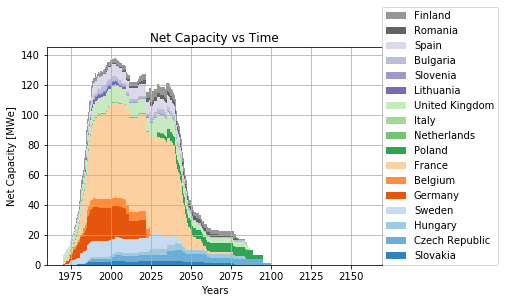
\includegraphics[scale=0.7]{./images/eu_future/power_plot.png}
	\end{center}
	\caption{Timeseries of installed nuclear capacity in \gls{EU}.}
	\label{fig:eu_pow}
\end{figure}
\FloatBarrier

\subsection{French \gls{SFR} Deployment Schedule}

Once \glspl{SFR} become available, in 2040,
600-MWe \glspl{SFR} are deployed to make up for the 
decommissioned \gls{LWR} capacities. 
This results in an installed capacity of 66,000 MWe
of \gls{SFR} by 2076, when the last \gls{LWR} decommissions.

\begin{figure}[htbp!]
        \begin{center}
                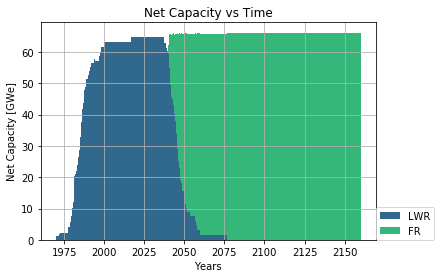
\includegraphics[scale=0.7]{./images/french-transition/power_plot.png}
        \end{center}
        \caption{French Transition into an SFR Fleet}
        \label{fig:sfr_num}
\end{figure}
\begin{figure}[htbp!]
	\begin{center}
		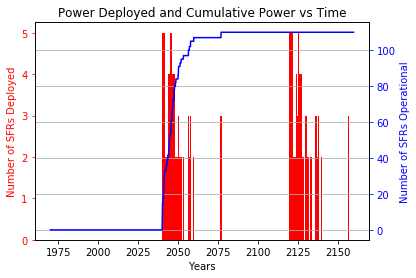
\includegraphics[scale=0.7]{./images/french-transition/sfr_deploy.png}
	\end{center}
	\caption{Deployment of French \glspl{SFR} and total installed capacity}
	\label{fig:dep}
\end{figure}
\FloatBarrier


\Cref{fig:sfr_num} and \cref{fig:dep} display
the French transition to \glspl{SFR} over time.
The steep transition from 2040 to 2060 reflects the scheduled
decommissioning of reactors built in the 1975-2000
era of aggressive nuclear growth in France.


\subsection{Material Definitions}
Depletion calculations of the nuclear fuel are recipe-based, such that a fresh 
and used fuel recipe is used for each reactor type.
For the compositions of the fuel, a reference depletion calculation
from ORIGEN is used (see \cref{tab:comp}). The recipe has also been used for
\cite{wilson_adoption_2009}.


\subsection{Scenario Descriptions}
The simulation follows the model fuel cycle, illustrated in \cref{diag:fc},
where a `source' provides natural uranium, which is enriched by an 'enrichment'
facility to produce \gls{UOX}, while disposing enrichment waste (tails)
to the 'sink' facility. The enriched \gls{UOX} fuels
the \gls{LWR}s and \gls{UOX} waste is produced. The used fuel
is sent to a pool to cool for 3 years \cite{carre_overview_2009}.
The cooled fuel is then reprocessed to separate plutonium and uranium,
or sent to a repository.
The plutonium mixed with depleted uranium (tails) makes \gls{MOX}.
The reprocessed uranium is unused and stockpiled. Uranium is reprocessed
in order to separate the raffinate (Minor actinides and fission products)
from 'usable' material. Though not utilized in this paper, reprocessed
uranium may substitute depleted uranium for \gls{MOX} production. In this
paper, there was sufficient depleted uranium inventory that using reprocessed
uranium was not considered. However, further in the future where the depleted
uranium inventory drains, reprocessed uranium (or, natural uranium) will need to be utilized. 


% Define block styles
\tikzstyle{decision} = [diamond, draw, fill=blue!20, 
text width=4.5em, text badly centered, node distance=3cm, inner sep=0pt]
\tikzstyle{block} = [rectangle, draw, fill=blue!20, 
text width=5em, text centered, rounded corners, minimum height=4em]
\tikzstyle{line} = [draw, -latex']
\tikzstyle{cloud} = [draw, ellipse,fill=red!20, node distance=3cm,
minimum height=2em]


\begin{figure}
        \centering
        \scalebox{0.7}{
                \begin{tikzpicture}[align=center, node distance = 3cm and 3cm, auto]
                % Place nodes
                \node [block] (sr) {Mine (\texttt{SOURCE})};
                \node [cloud, below of=sr] (nu) {Nat U};
                \node [block, below of=nu] (enr) {Enrichment ({\small \texttt{ENRICHMENT}})};
                \node [cloud, below of=enr] (uox) {\gls{UOX}};
                \node [block, below of=uox] (lwr) {\gls{LWR} (\texttt{REACTOR})};
                \node [cloud, right of=lwr] (snf) {\gls{UNF}};
                \node [cloud, right of=uox] (cunf) {Cooled \gls{UNF}};
                \node [block, right of=snf] (pool) {Pool (\texttt{Storage})};
                \node [cloud, left of=lwr] (tl2) {Dep U};
                \node [cloud, right of=enr] (tl) {Dep U};
                \node [block, right of=tl] (sk) {Repository (\texttt{SINK})};
                \node [cloud, below of=pool] (cunf2) {Cooled \gls{UNF}};
                \node [block, below of=snf] (rep) {Reprocessing ({\small \texttt{SEPARATIONS}})};
                \node [cloud, below of=rep] (u) {Sep. U} ;
                \node [cloud, left of=rep] (pu) {Sep. Pu};
                \node [block, left of=pu] (mix) {Fabrication (\texttt{MIXER})};
                \node [cloud, below of=mix] (mox) {\gls{MOX}};
                \node [block, below of=mox] (mxr) {\gls{MOX} Reactors};
                \node [cloud, right of= mxr] (snmox) {Spent \gls{MOX}};
                
                \draw[->, thick] (sr) -- (nu);
                \draw[->, thick] (nu) -- (enr);
                \draw[->, thick] (enr) -- (tl);
                \draw[->, thick] (enr) -- (tl2);
                \draw[->, thick] (tl) -- (sk);
                \draw[->, thick] (tl2) -- (mix);
                \draw[->, thick] (enr) -- (uox);
                \draw[->, thick] (uox) -- (lwr);
                \draw[->, thick] (lwr) -- (snf);
                
                \draw[->, thick] (lwr) -- (snf);
                \draw[->, thick] (snf) -- (pool);
                \draw[->, thick] (pool) -- (cunf);
                \draw[->, thick] (pool) -- (cunf2);
                \draw[->, thick] (cunf) -- (sk);
                \draw[->, thick] (cunf2) -- (rep);
                
                \draw[->, thick] (rep) -- (u);
                \draw[->, thick] (rep) -- (pu);
                \draw[->, thick] (pu) -- (mix);
                \draw[->, thick] (mix) -- (mox);
                \draw[->, thick] (mox) -- (mxr);
                \draw[->, thick] (mxr) -- (snmox);
                \draw[->, thick] (snmox) -- (rep);
                
                \end{tikzpicture}
        
                }
                \caption{Model Fuel Cycle with \gls{MOX} Reprocessing}
                \label{diag:fc}
\end{figure}


The second scenario separates plutonium from the \gls{UNF}
inventory from the previous simulation. The separated
plutonium mixed with the depleted uranium inventory from the previous simulation
creates \gls{MOX}, which fuels the \gls{SFR}s. 
\section{Scenario Specifications}
%% EARLY???

The scenario specifications for both simulations are
listed in tables \ref{tab:sim_eu} and \ref{tab:sim_france}.
The reprocessing and \gls{MOX} fabrication capacity for the 
first simulation are modeled after the 
French La Hague and MELOX site \cite{schneider_spent_2008, hugelmann_melox_1999}.

\begin{table}[h]
	\centering
	\begin{tabularx}{\textwidth}{bb}
		\hline
		\textbf{Specification} &\textbf{ Value} \\
		\hline
		Simulation Time & 1970-2050 \\ 
		Reprocessing Capacity & 91.6 MTHM of \gls{UNF} per month \cite{schneider_spent_2008} \\
		Reprocessing Efficiency & 99.8\% \\
		Reprocessing Streams & plutonium and uranium \\
		\gls{MOX} Fabrication & \small{9\% Reprocessed Pu + 91\% Depleted U} \\
		\gls{MOX} Fabrication Throughput & 16.25 MTHM of \gls{MOX} per month  \cite{hugelmann_melox_1999} \\
		\gls{MOX} Fuel Reprocessing Stage &  Used \gls{MOX} gets reprocessed infinitely. \\  
		Reprocessed Uranium Usage &  None. Stockpile reprocessed U \\
		\hline
	\end{tabularx}
	\caption {Specification for Historical Operation of \gls{EU} Case}
	\label{tab:sim_eu}
\end{table}

\begin{table}[h]
	\centering
	\begin{tabularx}{\textwidth}{bb}
		\hline
		\textbf{Specification }& \textbf{Value} \\
		\hline
		Simulation Time & 1970-2160 \\
		\gls{SFR} Available Year & 2040 \\
		\gls{UOX} Reprocessing Capacity & 20 tons per timestep \\
		\gls{MOX} Reprocessing Capacity & $\infty$ \\
		Reprocessing and Fabrication Begins & 2020 \\
		Separation Efficiency & 99.8 \% \\
		Reprocessing Streams & plutonium and uranium \\
		\small{Used \gls{UOX} and Depleted U Inventory} & 125,453 MTHM {\small (From first simulation)} \\
		\small{Additional Used \gls{UOX} or Depleted U} & None  \\
		\gls{MOX} Fabrication &  \small{11\% Reprocessed Pu + 89\% Depleted U}  \\
		\gls{MOX} Fabrication Throughput & infinite \\
		\gls{MOX} Fuel Reprocessing Stage &  Used \gls{MOX} gets reprocessed infinitely. \\
		Reprocessed Uranium Usage &  None. Stockpile reprocessed U. \\
		\hline
	\end{tabularx}
	\caption {Specification for French Transition to \gls{SFR} Case}
	\label{tab:sim_france}
\end{table}


\section{Reactor Specifications}
Three major reactors are used in the simulation, \gls{PWR}, \gls{BWR}, and ASTRID-type \gls{SFR}reactors.

For \glspl{LWR}, we used a linear core size model to capture
varying reactor capacity. For example, a 
1,200 MWe PWR has $193*\frac{1,200}{1,000} = 232$ \gls{UOX} assemblies, each
weighing 523.4 kg.
After each 18 month cycle, one-third of the 
core (77 assemblies) discharges. Refueling
is assumed to take 2 months to complete, during which the reactor
is shut down. This value is acquired by averaging the 
historical refueling outage. The specifications are defined in 
\Cref{tab:reactor-specs} details the reactor specifications in this simulation.

\begin{table}[h]
	\centering
	\begin{tabularx}{\textwidth}{blll}
		\hline
		\textbf{Specification} & \textbf{\gls{PWR} \cite{sutharshan_ap1000tm_2011}} & \textbf{\gls{BWR} \cite{hinds_next-generation_2006}} & \textbf{\gls{SFR}} \cite{varaine_pre-conceptual_2012}\\
		\hline
                Lifetime [y] & 60 & 60 & 80 \\
                Cycle Time [mos.]& 18 & 18 & 12\\ 
                Refueling Outage [mos.]& 2 & 2  & 2\\
                Rated Power [MWe] & 1000 & 1000 & 600\\
                Assembly mass [kg] & 523.4 & 180 & -- \\
                Batch mass [kg] & -- & -- & 5,568\\
                Discharge Burnup [GWd/tHM] & 51 & 51 & 105 \\
                Assemblies per core & 193  & 764 & -- \\
                Batches per core & 3 & 3 & 4\\
                Fuel & \gls{UOX} or \gls{MOX} & \gls{UOX} & \gls{MOX} \\
		\hline
	\end{tabularx}
        \caption {Model \gls{LWR} and \gls{ASTRID} specifications used for the simluations are listed, and \glspl{LWR} are modified
        linearly for varying power capacity. 
	\label{tab:reactor-specs}
	\end{table}

        \footnotetext{The simulated reactor lifetime reaches the licensed lifetime unless 
        the reactor is shut down prematurely.} 
        \footnotetext{Number of assemblies and corresponding \gls{LWR} core 
        masses are reported for a 1000MWe core. Reactors with different core  
        powers are modeled with a linear mass assumption.}
	
\FloatBarrier


\input{current}
\section{Future Nuclear Projections}

The future of nuclear energy in \gls{EU} nations is organized
in the table by the World Nuclear Association \cite{world_nuclear_association_nuclear_2017}.
We assumed that all the planned constructions 
are completed on their expected date without delay
or failure. Also, the newly constructed \glspl{LWR} are assumed to have a lifetime of 60 years.

\Cref{tab:eu_deployment} lists the reactors that are currently  planned or under construction.

 
\begin{table}[h]
	\centering
	
	\label{tab:eu_deployment}
	\scalebox{0.9}{
	\begin{tabular}{ccccc}
		\hline
		\textbf{Exp. Operational }&\textbf{ Country} &\textbf{ Reactor} & \textbf{Type} & \textbf{Gross MWe}\\
		\hline
		2018 & Slovakia  & Mochovce 3 & PWR & 440\\
		2018 & Slovakia & Mochovce 4 & PWR & 440 \\
		2018 & France & Flamanville 3 & PWR & 1600 \\
		2018 & Finland & Olkilouto 3 & PWR & 1720 \\		
		2019 & Romania & Cernavoda 3 & PHWR & 720 \\
		2020 & Romania & Cernavoda 4 & PHWR & 720 \\
		2024 & Finland & Hanhikivi & VVER1200 & 1200 \\
		2024 & Hungary & Paks 5 & VVER1200 & 1200 \\
		2025 & Hungary & Paks 6 & VVER1200 & 1200 \\
		2025 & Bulgaria & Kozloduy 7 & AP1000? & 950 \\
		2026 & UK & Hinkley Point C1 & EPR & 1670 \\
		2027 & UK & Hinkley Point C2 & EPR & 1670 \\
		2029 & Poland & Choczewo & N/A & 3000 \\
		2035 & Poland & N/A & N/A & 3000 \\
		2035 & Czech Rep & Dukovany 5 & N/A & 1200 \\
		2035 & Czech Rep & Temelin 3 & AP1000 & 1200 \\
		2040 & Czech Rep & Temelin 4 & AP1000 & 1200 \\
		\hline
	\end{tabular}
	}
	\caption {Power Reactors under construction and planned.
		Replicated from \cite{world_nuclear_association_nuclear_2017}.}
\end{table}
\FloatBarrier

For each \gls{EU} nation, the growth trajectory is categorized from
``Aggressive Growth'' to ``Aggressive Shutdown''. Aggressive growth is
characterized by a rigorous expansion of nuclear power while 
Aggressive Shutdown is characterized as a transition to rapidly
de-nuclearize the nation's electric grid. A nation's growth trajectory is
categorized into five degrees depending on G, the growth trajectory metric.
  
 \[
 G = \left\{\begin{array}{ll}
 \text{Aggressive Growth}, & \text{for } G \geq 2\\
 \text{Modest Growth}, & \text{for } 1.2 \leq G < 2\\
 \text{Maintanence}, & \text{for } 0.8 \leq G < 1.2 \\
 \text{Modest Reduction}, & \text{for } 0.5 \leq G< 0.8\\
 \text{Aggressive Reduction}, & \text{for } G \leq 0.5
 \end{array}\right\} = \frac{C_{2040}}{C_{2017}}\\\\
 \]
 \[
  G = \text{Growth Trajectory  } [-] 
 \]
 \[
 C_{i} = \text{Nuclear Capacity in Year i  } [MWe]
 \]
 
The growth trajectory and specific plan of each nation in the \gls{EU} 
is listed in Table \ref{tab:eu_growth}.

\begin{table}[h]
	\centering
		\begin{tabularx}{\textwidth}{lmb}
			\hline 
			
			\textbf{Nation} & \textbf{Growth Trajectory} & \textbf{Specific Plan }\\
			\hline
			UK & Aggressive Growth & {\small  13 units (17,900 MWe) by 2030.}\\
			\hline
			Poland & Aggressive Growth &  {\small Additional 6,000 MWe by 2035.}\\
			\hline
			Hungary & Aggressive Growth &  {\small Additional 2,400 MWe by 2025.} \\ 
			\hline
			Finland & Modest Growth &  {\small Additional 2,920 MWe by 2024.}\\
			\hline
			Bulgaria & Modest Growth &  {\small Additional 1,000 MWe by 2035.} \\
			\hline
			Romania & Modest Growth &  {\small Additional 1,440 MWe by 2020.} \\
			\hline
			Czech Rep. & Modest Growth & {\small  Additional 2,400 MWe by 2035.}\\
			\hline
			France & Modest Reduction & {\small No expansion or early shutdown.}\\
			\hline
			Spain & Modest Reduction &  {\small No expansion or early shutdown.} \\
			\hline
			Italy & Modest Reduction & {\small No expansion or early shutdown. }\\
			\hline
			Belgium & Aggressive Reduction & All shut down 2025.\\
			\hline
			Sweden & Aggressive Reduction & All shut down 2050.\\
			\hline
			Germany & Aggressive Reduction & All shut down by 2022.\\
			\hline
			
		\end{tabularx}

	\caption {Future Nuclear Programs of \gls{EU} Nations \cite{world_nuclear_association_nuclear_2017}}
  \label{tab:eu_growth}
\end{table}
\FloatBarrier

\section{Results}

First, we confirmed that France does not have enough
\gls{LWR} \gls{UNF} to transition into a fully \gls{SFR}
fleet. As shown in figure \ref{fig:only_france}, France
cannot meet the \gls{ASTRID} fuel demand without receiving
\gls{LWR} \gls{UNF} from other \gls{EU} nations. France
is able to fuel some of its \glspl{ASTRID} and breed more
plutonium, but cannot meet the fuel demand of 
all \glspl{ASTRID} with this aggressive deployment scheme.


\begin{figure}[htbp!]
	\begin{center}
		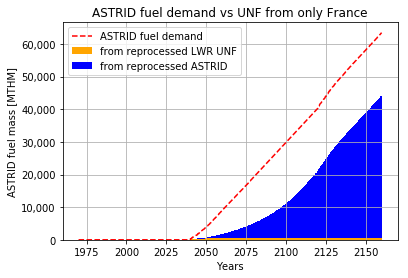
\includegraphics[scale=0.7]{./images/french-transition/france_only_compare.png}
	\end{center}
	\caption{\gls{ASTRID} fuel demand compared with fuel supply from only
			 France in the simulation. The lack of initial \gls{ASTRID} fuel
			 is caused by the lack of \gls{LWR} \gls{UNF} to reprocess. The
			 initial shortage then causes a decrease in plutonium bred by
			 \glspl{ASTRID}, thus a decrease in \gls{ASTRID} fuel supply.}
	\label{fig:only_france}
\end{figure}


\subsection{Nuclear Material Inventory}

Table \ref{tab:sim_result1} 
lists \gls{EU} material inventory in 2050.
The materials continue to accumulate after 2050, but the
\gls{UNF} France receives before 2050 is most impactful for the
feasibility of the transition. Note that table \ref{tab:sim_result1} 
distinguishes the
\gls{UOX} in the simulation either stored or reprocessed to create \gls{MOX}.


\begin{table}[h]
	\centering
        \caption{\gls{EU} nuclear material inventory in 2050.}
\begin{tabularx}{\textwidth}{XrX}
			\hline
                        \textbf{Category} & \textbf{Value} & Specifics \\
                                          & \textbf{[MTHM]} & \\ \hline
                        UOX Loaded  & 162,154 & UOX used in EU reactors 1970-2050\\ 
			MOX Loaded  & 6,685  & MOX used in French reactors 1970-2050\\
                        Available used UOX (EU)  & 95,193  & Used EU (minus France) 
                                UOX in storage for future ASTRID MOX 
                                production\\
                        Available used UOX (France) & 
                                12,494  & Used French UOX stored for 
                                future ASTRID MOX production. \\
                                Reprocessed UOX (France) & 51,382 & Used French UOX already reprocessed for the production of LWR MOX \\
			Tails  & 1,409,630  & (Tails generated) $-$ (Tails used for production of LWR MOX) \\ 
			Natural U Used  & 1,578,651  & \\ \hline
		\end{tabularx}
		
		\label{tab:sim_result1}
\end {table}
\FloatBarrier


Figures \ref{fig:eu_tail} and \ref{fig:eu_snf} show the 
accumulation of tails and used fuel over time in the \gls{EU}.
Tails accumulate as a by-product of uranium enrichment. 
Spent fuel is discharged from reactors every refueling period.
The entire core is discharged when the reactor decommissions.
A total of about $1,400,000$ MTHM of tails and $100,000$ MTHM of
\gls{UNF} have accumulated by 2050.
Figure \ref{fig:eu_fuel} shows the amount of fuel used in the \gls{EU}. The 
tails mass accumulation rate is fairly steady, with peaks occurring when new 
reactors are deployed.
In figure \ref{fig:eu_snf}, the peaks are caused by reactor decommissioning which 
triggers all the batches in the final reactor core to be sent to the repository.

\begin{figure}[htbp!]
	\begin{center}
		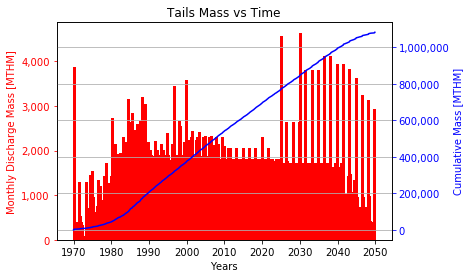
\includegraphics[scale=0.7]{./images/eu_future/tails.png}
	\end{center}
        \caption{Simulated accumulation of tails in the \gls{EU} is shown as a function of time.}
	\label{fig:eu_tail}
\end{figure}

\begin{figure}[htbp!]
	\begin{center}
		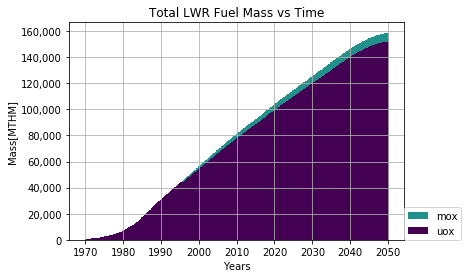
\includegraphics[scale=0.7]{./images/eu_future/total_fuel.png}
	\end{center}
\caption{Simulated total \gls{EU} fuel usage is shown as a function of time.}
	\label{fig:eu_fuel}
\end{figure}


\begin{figure}[htbp!]
	\begin{center}
			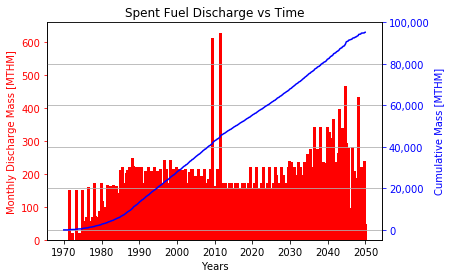
\includegraphics[scale=0.7]{./images/eu_future/snf_discharge.png}
	\end{center}
        \caption{Simulated \gls{EU} \gls{UNF} accumulation and discharge is 
shown as a function of time.}
	\label{fig:eu_snf}
\end{figure}


\subsection{French \gls{SFR} Deployment}
\FloatBarrier

Reprocessing the \gls{UNF} collected from all EU nations can provide
approximately 983 tons of plutonium. Table \ref{tab:pu} lists the 
isotope, mass fraction, and quantity of plutonium that can be obtained from the 
2050 \gls{UNF} inventory.  With the \gls{SFR} breeding ratio above one, France 
can transition into a fully \gls{SFR} fleet without extra construction of 
\glspl{LWR}. 

\begin{table}[h]
	\centering
	\caption{Plutonium in the \gls{UNF} inventory.}
	\begin{tabular}{lrr}
		\hline
		\textbf{Isotope} & \textbf{Mass Fraction in Used Fuel [\%]} & \textbf{Quantity [t]} \\ \hline
		Pu238 & 0.0111 & 10.52 \\ 
		Pu239 & 0.518 & 545.05 \\ 
		Pu240 & 0.232 & 244.11 \\ 
		Pu241 & 0.126 & 132.58 \\ 
		Pu242 & 0.0487 & 51.24 \\ \hline
		\textbf{Total} & \textbf{0.9358} & \textbf{983.52} \\ \hline
	\end{tabular}
	
	\label{tab:pu}
\end{table}

From Varaine et al. \cite{varaine_pre-conceptual_2012}, a French
ASTRID-type 600\gls{MWe} \gls{SFR} consumes $1.125$ metric tons of
plutonium a year, with an initial plutonium loading of $4.9$ metric tons.
 
Used \gls{MOX} from an ASTRID reactor is 23.95\% plutonium
in this simulation (see table \ref{tab:comp_fresh}), whereas fresh \gls{MOX} is 22\% plutonium.
The plutonium breeding ratio in this simulation is thus assumed to be
$\approx 1.08$.

Figure \ref{fig:fuel} shows \gls{MOX} loaded in the \glspl{SFR} per month.  The plot 
has peaks during a period of aggressive deployment of \glspl{SFR} followed by 
an equilibrium at 100 \gls{MTHM}. The peaks reoccur with the deployment of the 
second generation of \glspl{SFR}.  The spikes are due to initial fuel demand 
corresponding to these new deployments.  The initial cores loaded into new 
\glspl{SFR} rely on the \gls{MOX} created from legacy \gls{UNF}. Once the 
deployed \glspl{SFR} create enough extra plutonium, the legacy \gls{UNF} is no 
longer used. Notably, this switch from a less preferred fuel origin to a more 
preferred fuel origin is handled automatically within \Cyclus via user-defined preferences 
within its dynamic resource exchange algorithm \cite{gidden_methodology_2016}.


\begin{figure}[htbp!]
	\begin{center}
		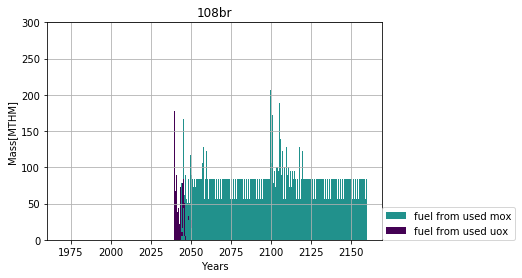
\includegraphics[width=1.0\textwidth]{./images/french-transition/where_fuel.png}
	\end{center}
	\caption{Fuel loaded into \glspl{SFR} was simulated in discrete 
        batches.}
	\label{fig:fuel}
\end{figure}

Figure \ref{fig:pu_no_cum} shows the separated plutonium discharge per 
month from the reprocessing plant. The plutonium outflux does not precisely 
follow the fuel demand because \Cyclus agents have material buffers that 
store commodity fuel for later usage. The reprocessed plutonium from legacy 
\gls{UNF} is stored for the initial loading of \glspl{SFR}.  Plutonium separated 
from legacy \gls{UNF} meets plutonium demands sufficiently to reduce the 
reprocessing demand for the first aggressive deployment of \glspl{SFR}.  
The plutonium from reprocessing legacy fuel is a flat rectangle because the 
reprocessing throughput was set to 183.2 $\frac{\gls{MTHM}}{month}$ to 
avoid reprocessing all the legacy in one timestep. 
 

\begin{figure}[htbp!]
	\begin{center}
		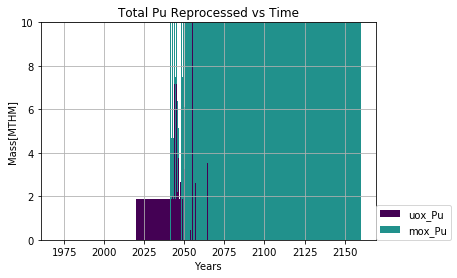
\includegraphics[scale=0.7]{./images/french-transition/pu.png}
	\end{center}
	\caption{The separated plutonium discharge from the reprocessing plant 
        in $\frac{\mbox{MTHM}}{\mbox{month}}$.}
	\label{fig:pu_no_cum}
\end{figure}

 Table \ref{tab:sfr_sim_result} lists French reprocessing and 
 \gls{ASTRID} fuel fabrication metrics.

\begin{table}[h]
	\centering
	\caption {In the French transition to \glspl{SFR},
				  the total legacy \gls{UNF} reprocessed is the 
                                  amount of \gls{UNF} France needs 
				  for a transition into a fully \gls{SFR} fleet. 
                          }
	\scalebox{0.86}{
		\begin{tabular}{llr}
			\hline
			\textbf{Category} & \textbf{Unit} & \textbf{Value}  \\ \hline
			Total \gls{ASTRID} MOX used & MTHM & 63,452  \\ 
			\textbf{Average UOX Reprocessing} & MTHM/month & \textbf{124.6} \\
			\textbf{Average Total Reprocessing} & MTHM/month & \textbf{63.23} \\
			\textbf{Average Fuel Fabrication} & MTHM/month & \textbf{45.32} \\
			Total \glspl{SFR} Deployed & & 220 \\ 
			Total Plutonium Reprocessed & MTHM & 14,620 \\ 
			Total \gls{ASTRID} fuel from UOX Waste & MTHM & 2,856  \\ 
			Total \gls{ASTRID} fuel from MOX Waste & MTHM  & 60,596 \\ 
			Total Tails used & MTHM & 49,492 \\ 
			\textbf{Total legacy UNF reprocessed} & MTHM & \textbf{52,874} \\ 
			Total Reprocessed Uranium Stockpile & MTHM & 148,620 \\ 
			Total Raffinate & MTHM & 17,901 \\ \hline
		\end{tabular}}
		
		\label{tab:sfr_sim_result}
\end {table}


These results demonstrate that despite the large amount of initial plutonium that has to be reprocessed
prior to \gls{ASTRID} deployment, the 20 years (2020-2040) of 
\gls{ASTRID} fuel preparation
allows a reasonable level of average
\gls{UOX} reprocessing capacity demand. \gls{UOX} reprocessing continues 
until 2057, when the \gls{ASTRID} spent fuel can supply the plutonium
for its own fuel.


\section{Discussion}
This work demonstrated that, given infinite
reprocessing and \gls{MOX} fabrication capacities,
France, by receiving \gls{UNF} from other \gls{EU} nations,
 can transition into, for unchanging nuclear electricity demand,
a fully \gls{SFR} fleet
with installed capacity of 60,000 MWe by 2076.
\gls{MOX} from reprocessed \gls{UNF} meets the initial fuel demand,
which later on is supplied by \gls{MOX} created from recycled \gls{MOX}.

Since most \gls{EU} nations do not have an operating \gls{UNF}
repository or a management plan, they have a strong incentive
to send all their \gls{UNF} to France. The nations
with aggressive nuclear reduction can phase out nuclear
without constructing a High Level Waste repository. France has an
incentive to take this fuel, since reuse of used fuel from
other nations will allow France to meet their MOX demand
without new construction of \glspl{LWR}.

Though complex political and economic factors are not
addressed, and various assumptions present for this scenario,
this option may hold value for the \gls{EU} as a nuclear community,
and for France to advance into a closed fuel cycle.



\bibliographystyle{abbrv}
\bibliography{./bibliography.bib}

\section{Fresh and Used Fuel Composition}
\begin{table}[h]
	\centering
	\scalebox{0.75}{
		\begin{tabular}{|c|c|c|c|c|c|c|}
		\hline
		 Isotope 	 & 	Fresh UOX Fuel & 	Spent UOX Fuel (BU: $51\frac{GWdth}{MTHM}$) & Fresh SFR Fuel & Spent SFR Fuel \\ \hline 
		 He4	 & 	 	& 	9.474E-07 & 	 	 & 	7.827E-06 \\ \hline 
		 Ra226	 & 	 	& 	9.788E-14 & 	 	 & 	5.151E-14 \\ \hline 
		 Ra228	 & 	 	& 	2.750E-20 & 	 	 & 	4.904E-21 \\ \hline 
		 Pb206	 & 	 	& 	5.574E-18 & 	 	 & 	1.210E-18 \\ \hline 
		 Pb207	 & 	 	& 	1.685E-15 & 	 	 & 	1.892E-16 \\ \hline 
		 Pb208	 & 	 	& 	3.688E-12 & 	 	 & 	5.875E-11 \\ \hline 
		 Pb210	 & 	 	& 	3.023E-19 & 	 	 & 	8.143E-18 \\ \hline 
		 Th228	 & 	 	& 	8.475E-12 & 	 	 & 	1.004E-10 \\ \hline 
		 Th229	 & 	 	& 	2.727E-12 & 	 	 & 	4.065E-12 \\ \hline 
		 Th230	 & 	 	& 	2.625E-09 & 	 	 & 	2.139E-09 \\ \hline 
		 Th232	 & 	 	& 	4.174E-10 & 	 	 & 	4.425E-11 \\ \hline 
		 Bi209	 & 	 	& 	6.607E-16 & 	 	 & 	2.600E-14 \\ \hline 
		 Ac227	 & 	 	& 	3.096E-14 & 	 	 & 	4.840E-15 \\ \hline 
		 Pa231	 & 	 	& 	9.246E-10 & 	 	 & 	1.300E-10 \\ \hline 
		 U232	 & 	 	& 	0.000 & 	 	 & 	0.000 \\ \hline 
		 U233	 & 	 	& 	2.213E-09 & 	 	 & 	5.528E-09 \\ \hline 
		 U234	 & 	0.000& 	0.000 & 	 	 & 	0.000 \\ \hline 
		 U235	 & 	0.032& 	0.007 & 	0.002 & 	0.000 \\ \hline 
		 U236	 & 	 	& 	0.005 & 	 	 & 	0.000 \\ \hline 
		 U238	 & 	0.968& 	0.920 & 	0.887 & 	0.808 \\ \hline 
		 Np237	 & 	 	& 	0.000 & 	 	 & 	0.000 \\ \hline 
		 Pu238	 & 	 	& 	0.000 & 	0.001 & 	0.001 \\ \hline 
		 Pu239	 & 	 	& 	0.006 & 	0.060 & 	0.085 \\ \hline 
		 Pu240	 & 	 	& 	0.002 & 	0.027 & 	0.027 \\ \hline 
		 Pu241	 & 	 	& 	0.001 & 	0.014 & 	0.003 \\ \hline 
		 Pu242	 & 	 	& 	0.000 & 	0.005 & 	0.001 \\ \hline 
		 Pu244	 & 	 	& 	2.864E-08 & 1.508E-07 & 	5.461E-09 \\ \hline 
		 Am241	 & 	 	& 	6.442E-05 & 	 	 & 	0.001 \\ \hline 
		 Am242m	 & 	 	& 	8.533E-07 & 	 	 & 	7.961E-05 \\ \hline 
		 Am243	 & 	 	& 	0.000 & 	 	 & 	0.000 \\ \hline 
		 Cm242	 & 	 	& 	2.589E-05 & 	 	 & 	5.331E-05 \\ \hline 
		 Cm243	 & 	 	& 	0.000 & 	 	 & 	3.242E-06 \\ \hline 
		 Cm244	 & 	 	& 	8.561E-05 & 	 	 & 	0.000 \\ \hline 
		 Cm245	 & 	 	& 	5.721E-06 & 	 	 & 	3.936E-05 \\ \hline 
		 Cm246	 & 	 	& 	7.295E-07 & 	 	 & 	1.434E-05 \\ \hline 
		 Cm247	 & 	 	& 	0.000 & 	 	 & 	5.317E-07 \\ \hline 
		 Cm248	 & 	 	& 	7.691E-10 & 	 	 & 	0.000 \\ \hline 
		 Cm250	 & 	 	& 	4.280E-18 & 	 	 & 	6.407E-15 \\ \hline 
		 Cf249	 & 	 	& 	1.649E-12 & 	 	 & 	6.446E-10 \\ \hline 
		 Cf250	 & 	 	& 	2.041E-12 & 	 	 & 	6.703E-11 \\ \hline 
		 Cf251	 & 	 	& 	9.865E-13 & 	 	 & 	1.903E-12 \\ \hline 
		 Cf 252	 & 	 	& 	6.579E-13 & 	 	 & 	4.014E-14 \\ \hline 
		 H3	 & 	 	& 	8.584E-08 & 	 	 & 	1.747E-07 \\ \hline 
		 C14	 & 	 	& 	4.057E-11 & 	 	 & 	 	 \\ \hline 
		 C Other	 & 	 	& 	 	 & 	 	 & 	 	 \\ \hline 
		 Kr81	 & 	 	& 	4.216E-11 & 	 	 & 	8.038E-12 \\ \hline 
		 Kr85	 & 	 	& 	3.444E-05 & 	 	 & 	2.950E-05 \\ \hline 
		 Kr Other	 & 	 	& 	0.000 & 	 	 & 	0.000 \\ \hline 
		 Sr90	 & 	 	& 	0.001 & 	 	 & 	0.001 \\ \hline 
		 Sr Other	 & 	 	& 	0.000 & 	 	 & 	0.000 \\ \hline 
		 Tc99	 & 	 	& 	0.000 & 	 	 & 	5.391E-05 \\ \hline 
		 Tc Other	 & 	 	& 	0.000 & 	 	 & 	0.002 \\ \hline 

		\end{tabular}}
		\caption{Fresh and Spent Fuel Compositions}
		\label{tab:comp}
\end {table}


\end{document}
